\documentclass[11pt]{article}

\usepackage[a4paper, total={16cm, 24cm}]{geometry}
\usepackage[portuguese]{babel}
\usepackage[utf8]{inputenc}
\usepackage{graphicx}
\usepackage{amsmath}
\usepackage{tikz}
    \usetikzlibrary{shadows}
\usepackage{booktabs}
\usepackage[colorlinks=true]{hyperref}
\usepackage{listings}
    \renewcommand\lstlistingname{Listagem}
    \lstset{numbers=left, numberstyle=\tiny, numbersep=5pt, basicstyle=\footnotesize\ttfamily, frame=tb,rulesepcolor=\color{gray}, breaklines=true}
\usepackage{blindtext}
\usepackage[export]{adjustbox}

% -------------------------------------------------------------------------------------------
\title
{
    
\includegraphics[width=0.4\textwidth]{images/ue_logo.png}
    \\[0.1cm]
    \textbf{Serviço de Mensagens Curtas Inteligente} \\
    Estrutura de Dados e Algoritmos I
}

\author
{
    \textbf{Professora:} Lígia Ferreira, Teresa Gonçalves \\
    \textbf{Realizado por:} Miguel de Carvalho (43108), Ricardo Oliveira (42647)
}
\date{\today}

% -------------------------------------------------------------------------------------------
%                                Body                                                       %
% -------------------------------------------------------------------------------------------

\begin{document}
\maketitle

% -------------------------------------------------------------------------------------------
\section{Introdução}

\hspace{0,5cm}Neste trabalho foi solicitado a realização de um programa que simule o \textbf{Serviço de Mensagens Curtas Inteligentes}, ou seja, que implemente a tecnologia de escrita de mensagens curtas inteligente T9 (Text on 9 Keys), que está representada na figura abaixo.

\begin{figure}[h!]
    \begin{center}
        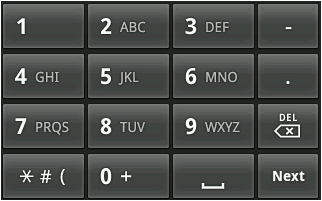
\includegraphics[width=0.6\textwidth]{images/t9_keys.png}
        \caption{Modelo de 3 Estados}
    \end{center}
\end{figure}

Esta tecnologia permite que o utilizador escreva palavras através das teclas numéricas. Cada tecla corresponde a 3 ou 4 letras do alfabeto e através de um dicionário é possível formar uma palavra através dos algarismos correspondentes a cada uma das suas letras.

Por exemplo quando o  utilizador clicar nas teclas, seguindo a sequência, \verb|66836|, o utilizador poderá querer formar a palavra \textbf{movem} ou a palavra \textbf{ontem}.
% -------------------------------------------------------------------------------------------
\section{Implementação}

\hspace{0,5cm}Inicialmente pensámos como deveríamos proceder para realizar o trabalho e chegámos à conclusão de que era apenas necessário utilizar duas \textbf{hashtables} para guardar o \textbf{teclado K9} e outra para guardar o \textbf{dicionário} que continha as palavras que o utilizador poderia formar através das suas \textbf{sequências introduzidas}.

No início o programa cria uma \textbf{hashtable} denominada \verb|T9| com um espaço de 11 e outra \textbf{hashtable} denominada \verb|Dictionary| com um espaço de 10 milhões. Após a criação de ambas as \textbf{hashtables} é realizada uma verificação para perceber se o ficheiro que o utilizador passou como argumento existe. De seguida são inseridos os algarismos correspondentes às letras na \textbf{hashtable} \verb|T9|. Além disso, o programa percorre o ficheiro linha a linha, ou seja, cada palavra e insere cada uma delas na \textbf{hashtable} \verb|Dictionary|, usando a \textbf{sequência de caracteres} para calcular a \textbf{hash da palavra}. Assim, palavras que tenham a mesma \textbf{sequência de caracteres} irão estar na mesmo \textbf{posição}. Por fim, o utilizador insere a \textbf{sequência de caracteres}, o programa calcula o \textbf{hash} da palavra e acede a essa \textbf{posição na hashtable} e retorna todas as palavras que correspondam a essa \textbf{sequência de caracteres} introduzida pelo utilizador.

% -------------------------------------------------------------------------------------------
\section{Execução}

\hspace{0,5cm}Para executar o \textbf{Serviço de Mensagens Curtas Inteligente}, o utilizador deverá passar como argumento o \textbf{dicionário (ficheiro com as palavras)}.
\par Exemplo:
\begin{lstlisting}[language=bash]
  $ gcc -lm -Wextra -Wall -o .compiled main.c hashtable.c
  $ ./.compiled dictionaries/portuguese-large_lower.txt
  ** Escreva a sua mensagem **
  66836
  Sugestao: movem, aceita (s/n)? n
  Sugestao: ontem, aceita (s/n)? s
  62834834
  Sugestao: naveguei, aceita (s/n)? s
  62
  Sugestao: ma, aceita (s/n)? n
  Sugestao: na, aceita (s/n)? s
  932
  Nao existem mais sugestoes; introduza a palavra do teclado.
  web
  1
  Mensagem: ontem naveguei na web
  0
  Deseja sair da aplicacao (s/n)? s
\end{lstlisting}

% -------------------------------------------------------------------------------------------
\section{Limitações e Soluções}

O nosso programa apresenta 2 limitações, não interpreta palavras que contenham \textbf{letras maiúsculas} e palavras que contenham \textbf{caracteres especiais}.

\subsection{Palavras com Letras Maiúsculas}

Como a tabela de correspondências dos algarismos correspondentes às letras (T9) não apresenta letras maiúsculas, para solucionarmos esta situação, \textbf{convertemos} todas as palavras dos dicionários para \textbf{letras minúsculas}, já que o programa não iria interpretar as \textbf{letras maiúsculas}.

\subsection{Palavras com Caracteres Especiais}

A tabela de correspondências dos algarismos correspondentes às letras (T9) não contem caracteres especiais tal como \verb|'|, para solucionarmos esta situação, decidimos que o programa iria ignorar esses caracteres.

% -------------------------------------------------------------------------------------------
\section{Conclusão}

\hspace{0,5cm}Em suma, com a realização deste trabalho \textbf{"Serviço de Mensagens Curtas Inteligente"} ficámos muito mais esclarecidos sobre o seu modo de funcionamento e quais as componentes necessárias para ter um sistema destes operacional.

Saliento também que nos ajudou a entender melhor como funcionam as \textbf{Hashtables} e as suas \textbf{funções de manipulação}, tais como, inserção, remoção e a listagem.
% -------------------------------------------------------------------------------------------
\section{Comentários Adicionais}

\hspace{0,5cm}No início da realização deste trabalho deparámos-nos com grandes dificuldades em conseguirmos manipular as palavras provenientes do \textbf{dicionário e do teclado K9}, pois por padrão a linguagem \textbf{C} usa \textbf{ASCII}, que não contêm todos o caracteres especiais que estão no \textbf{dicionário de palavras e no teclado K9}, foi então necessário substituirmos o \verb|char| pelo \verb|wchar_t| , pois o \verb|wchar_t| está preparado para lidar com estes caracteres especiais.

Deparámos-nos também com alguns problemas relacionados com o uso do tipo \verb|int| para guardar a sequência de caracteres correspondente a cada palavra, pois não era possível guardar a sequência correspondente a palavras com 38 caracteres. Para solucionar esta situação usámos variáveis do tipo \verb|unsigned long|.
% -------------------------------------------------------------------------------------------
\end{document}